\documentclass[a4paper]{report}
\usepackage{amsmath,amssymb,bm,caption,enumerate,float,geometry,graphicx,indentfirst,setspace}
\geometry{left=4.5cm,right=4.5cm,top=4cm,bottom=4cm}
\captionsetup[figure]{labelsep=period}
\begin{document}
	\renewcommand\thesection{\arabic{section}}
	\begin{Large}
		\begin{center}
			\setlength{\baselineskip}{14pt}
			\vspace{1.25cm}
			\rule[0cm]{11.2cm}{0.03em}\\
			\vspace{0.5cm}
			\textsc{UM-SJTU Joint Institute}\\
			\vspace{0.25cm}
			\textsc{Physics Laboratory\\(Vp141)}
			\vspace{0.3cm}
			\rule[0cm]{11.8cm}{0.05em}
			\vspace{4.9cm}\\
			\textsc{Laboratory Report}
		\end{center}
	\end{Large}
	\vspace{0.85cm}
	\begin{large}
		\begin{center}
			\textsc{Exercise 4}
			\\~
			\textsc{Measurement of the Speed of Sound}
		\end{center}
		\vspace{6cm}
	\end{large}
	\begin{tabular}{l l l}
	Name: Yihua Liu&ID:518021910998&Group 9\\
	Name: Guanghan Xi&ID:518021910778&Group 9\\
	&&\\
	Date: 16 June 2019&&\\
	\end{tabular}
	\thispagestyle{empty}
	\newpage
	\section{Introduction}
	The Objective of the experiment was to measure the speed of sound in air and water by three methods, including the resonance method, the phase comparison method, and the time difference methods. During the measurement, we will learn how to use function generators and oscilloscopes.
	
	Sound is a kind of longitudinal waves in media like air, waterand solids, also called compression waves, which the displacement of the medium is in either the same direction as or the opposite direction to the direction of propagation of the wave.
	
	The relation among the phase speed $v$, the frequency $f$, and the length $\lambda$ can be expressed by
	\begin{equation}
	v=\lambda f
	\end{equation}
	
	Besides, the motion of the wave is identical to one-dimension motion, so we have
	\begin{equation}
	L=vt
	\end{equation}
	
	If we want to measure the speed of sound using an oscilloscope, we should observe a maximum output power in the oscillograph, when
	\begin{equation}
	L=n\dfrac{\lambda}{2}
	\end{equation}
	
	This is because at these moments, the standing waves will form so that we can measure the maximum value of power. As the length of wave increases, the signal voltage periodically decreases for every half of $\lambda$.
	
	As for the phase-comparison method, we want to use Lissajous figures to describe harmonic motions. In this part, the position vector can be expressed by
	\begin{equation}
	\bm{r}(t)=(A_x\cos(\omega_xt+\phi_x),A_y\cos(\omega_yt+\phi_y))
	\end{equation}
	
	Generally, the figure will show two elliptical arcs. However, when $\omega_x=\omega_y$ and $\vert\phi_x-\phi_y\vert=n\Pi$, where $n=0,1,2,...$, the trajectories will become a superimposed straight line. Consequently, these points L has the relationship with the wavelength that
	\begin{equation}
	L=n\lambda
	\end{equation}
	where $n=1,2,...$.
	
	Alternatively, we can directly read the length and the time period and derive the speed of sound by Equation 2. To measure $L$ and $t$, we need to use the wave source $S_1$ and the receiver $S_2$ to transfer ultrasonic pulse signals in water, then $L$ is the distance between $S_!$ and $S_2$, which is quite trivial.
	\section{Experimental setup}
	To thoroughly complete measurement for three methods, we use a signal source, two piezoelectric transducers $S_1$ and $S_2$, and an oscilloscope as is shown in Figure 1.
	\begin{figure}[H]
		\centering
		\includegraphics[width=0.8\linewidth]{1.png}
		\caption{Experimental setup.}
		\label{fig:1}
	\end{figure}
	The wave is sent from $S_1$ and it is received and reflected by $S_2$. The two elements should be arranged parallel to each other to make sure the wave can be transmitted properly. We can use the micrometer caliper set on the right side of the equipment to adjust the distance between the two elements.
	
	We can adjust the frequency and the width by pushing function buttons. The uncertainty of the length is 0.001 mm. When adjusting the scale of the graph both horizontally and vertically, the uncertainty of the length changes.
	
	By switching the mode, we can view Lissajous fiures on the screen. There are two optional channels on the upper-left and upper-right side respectively. In this part, we can choose Channel 1. There is another button that can adjust the two reference lines.
	\section{Measurements}
	\subsection{Resonance Method}
	\begin{enumerate}[1.]
		\item Set the distance between $S_1$ and $S_2$ at approximately but more than 1 cm.
		\item Turn on the power of the signal source and the oscilloscope to initialize.
		\item Choose \textit{Continuous} wave for \textit{Method}.
		\item Adjust \textit{Signal Strength} until a 10 V peak voltage is shown on the oscilloscope.
		\item Adjust \textit{Signal Frequency} between 34.5 KHz and 40 KHz until the maximum peak-to-peak voltage is reached and record the signal frequency.
		\item Gradually increase $L$ gradually by moving $S_2$ until there is obvious change in value. Observe the corresponding output voltage of $S_2$ on the oscilloscope and the position of $S_2$ as $L_2$ when the maximum output voltage is reached.
		\item Repeat Step 6 to record 12 values of $L_2$ and find $v$ by performing a linear fit to the data.
	\end{enumerate}

	The above measurement of the length was repeated for 12 times and the obtained data was presented in Table 1.
	
	Since there are noises when measuring the length and the vertical scale is not precise enough, it is difficult to lock the oscilloscope at the actual maximum value. The uncertainty of this measurement is larger than the uncertainty of the length observed on the oscilloscope.
	\subsection{Phase-comparison Method}
	\begin{enumerate}[1.]
		\item Change the mode to view Lissajous figures.
		\item Reset the distance between the transimitted and the received signals.
		\item Move $S_2$ and record the position when the Lissajous figure becomes a straight line with the same direction of slope, ignoring the asymmetric ones.
		\item Repeat Step 3 to collect 12 sets of data and perform a linear fit to find $v$.
	\end{enumerate}

	In the measurement above, we can find that as the distance increases, the amplitude of the graph decreses, and when Lissajous figure is going to reach the status of a straight line, the adjustment of the micrometer caliper is so sensitive to the change of the graph that one straight line might be missed during adjustment. In this case, it has to be dismissed and record next time it becomes a straight line. Besides, to avoid missing anyone, the straight line might not be precisely formed when recording. When one reading is determined, the graph on the oscilloscope still changes a little around the straight line and flat elliptical shapes.
	\subsection{Time-difference Method (Liquid)}
	\begin{enumerate}[1.]
		\item Reset the mode of figures and the distance between $S_1$ and $S_2$ greater than 10 cm.
		\item Change the medium from air to water.
		\item Adjust the frequency to 100 Hz and the width to 500 $\mu$s.
		\item Move $S_2$ and measure the time and the distance between the starting points of neighboring periods through the cursor function of the oscilloscope.
		\item Repeat Step 4 to record 12 pairs of data and perform a linear fit to find $v_{\rm water}$.
	\end{enumerate}

	Since $S_1$ is the signal source and $S_2$ is for receiving the signal, there is no need to double or half the distance. Changing the frequency and the width may lead to change in scale so that the shape of the wave is out of the range of the current scale of the oscilloscope. The sound in water is much faster than in air, so each increment in the distance between $S_1$ and $S_2$ will be more.
	\section{Results}
	\subsection{Measurements of the speed of sound by resonance method}
	The frequency of the sound wave $f=38.500$ kHz. The temperature $T=22 ^\circ {\rm C} \pm 1 ^\circ {\rm C}$.
	The distances between $S_1$ and $S_2$ were measured in the procedure described in section 3.1 and the linear fit from $L_i$ can be derived from Table 1.
	\begin{tabular}{|c|c||c|c|}
		\hline
		Measurement&$L_i$ [mm]$\pm$0.001[mm]&Measurement&$L_i$ [mm]$\pm$0.001[mm]\\
		\hline
		1&14.619&7&41.678\\
		\hline
		2&18.835&8&46.225\\
		\hline
		3&23.310&9&50.864\\
		\hline
		4&27.968&10&55.364\\
		\hline
		5&32.567&11&59.999\\
		\hline
		6&37.060&12&64.530\\
		\hline
	\end{tabular}
	\begin{center}
		Table 1. Data table for the resonance method.
	\end{center}
	By Equation 3, the value of the distance $L$ is linear to the wavelength $\lambda$, which is presented in Figure 2. After a statistical test is run in order to test a hypothesis there is a linear relation between the two quantities as is considered and nothing yield to reject this hypothesis, we fit a straight line $L=\alpha \lambda+\beta$ to the data. It turns out that the slope $\alpha=4.559$ mm and the intercept $\beta=9.783$ mm with standard errors $u_\alpha=0.009$ mm and $u_\beta=0.068$ mm and $R^2$=0.99996. The fitting procedure are performed using Origin.
	Using the value of the slope from the linear relation Equation 3, the speed of sound $v$ can be found as
	\begin{equation}
	v=\lambda f=2\alpha f=2\dot{4.559}\dot{38.500}=351.043\pm0.107\ \rm{m/s}
	\end{equation}
	with the relative uncertainty 0.03\%.
		\begin{figure}[H]
		\centering
		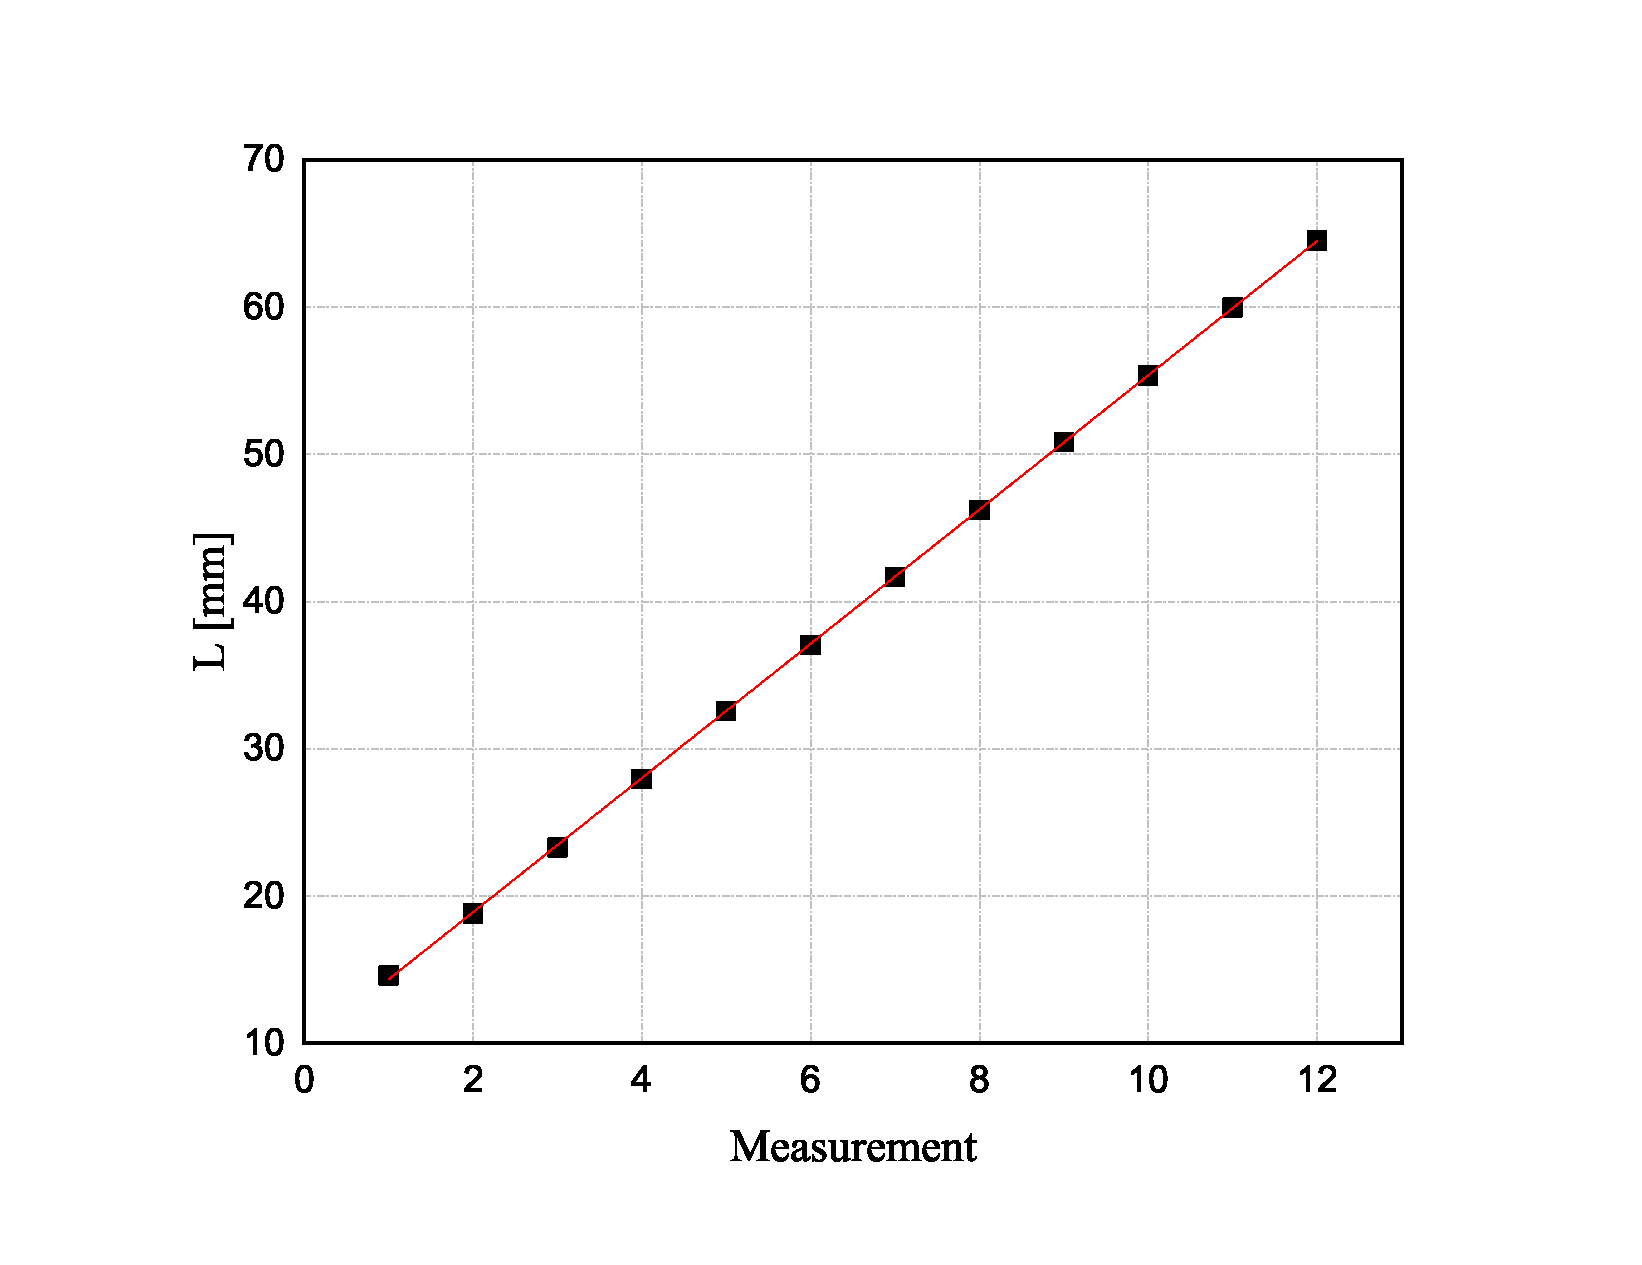
\includegraphics[width=0.8\linewidth]{2.eps}
		\caption{Measurement data with error bars and a linear fit to the data for the relation between the distance and the measurement. The value of $R^2$ for the obtained fit is 0.99996.}
		\label{fig:2}
	\end{figure}
	\subsection{Measurements of the speed of sound by phase-comparison method}
	The distances between $S_1$ and $S_2$ were measured in the procedure described in section 3.2 and the linear fit from $L_i$ can be derived from Table 2.
	\begin{tabular}{|c|c||c|c|}
		\hline
		Measurement&$L_i$ [mm]$\pm$0.001[mm]&Measurement&$L_i$ [mm]$\pm$0.001[mm]\\
		\hline
		1&14.120&7&68.735\\
		\hline
		2&23.251&8&77.721\\
		\hline
		3&32.319&9&86.751\\
		\hline
		4&41.562&10&95.816\\
		\hline
		5&50.614&11&104.910\\
		\hline
		6&59.680&12&113.956\\
		\hline
	\end{tabular}
	\begin{center}
		Table 2. Data table for the phase comparison method.
	\end{center}
	By Equation 5, the value of the distance $L$ is linear to the wavelength $\lambda$, which is presented in Figure 3. After a statistical test whose results satisfy the hypothesis of linear relation, we fit a straight line $L=\alpha \lambda+\beta$ to the data. By linear fitting, the slope $\alpha=9.070$ mm and the intercept $\beta=5.167$ mm with standard errors $u_\alpha=0.007$ mm and $u_\beta=0.050$ mm and $R^2$=0.99999. The fitting procedure are performed using Origin.
	Using the value of the slope from the linear relation Equation 3, the speed of sound $v$ can be found as
	\begin{equation}
	v=\lambda f=\alpha f=9.070\dot{38.500}=349.195\pm0.041\  \rm{m/s}
	\end{equation}
	with the relative uncertainty 0.01\%.
	\begin{figure}[H]
		\centering
		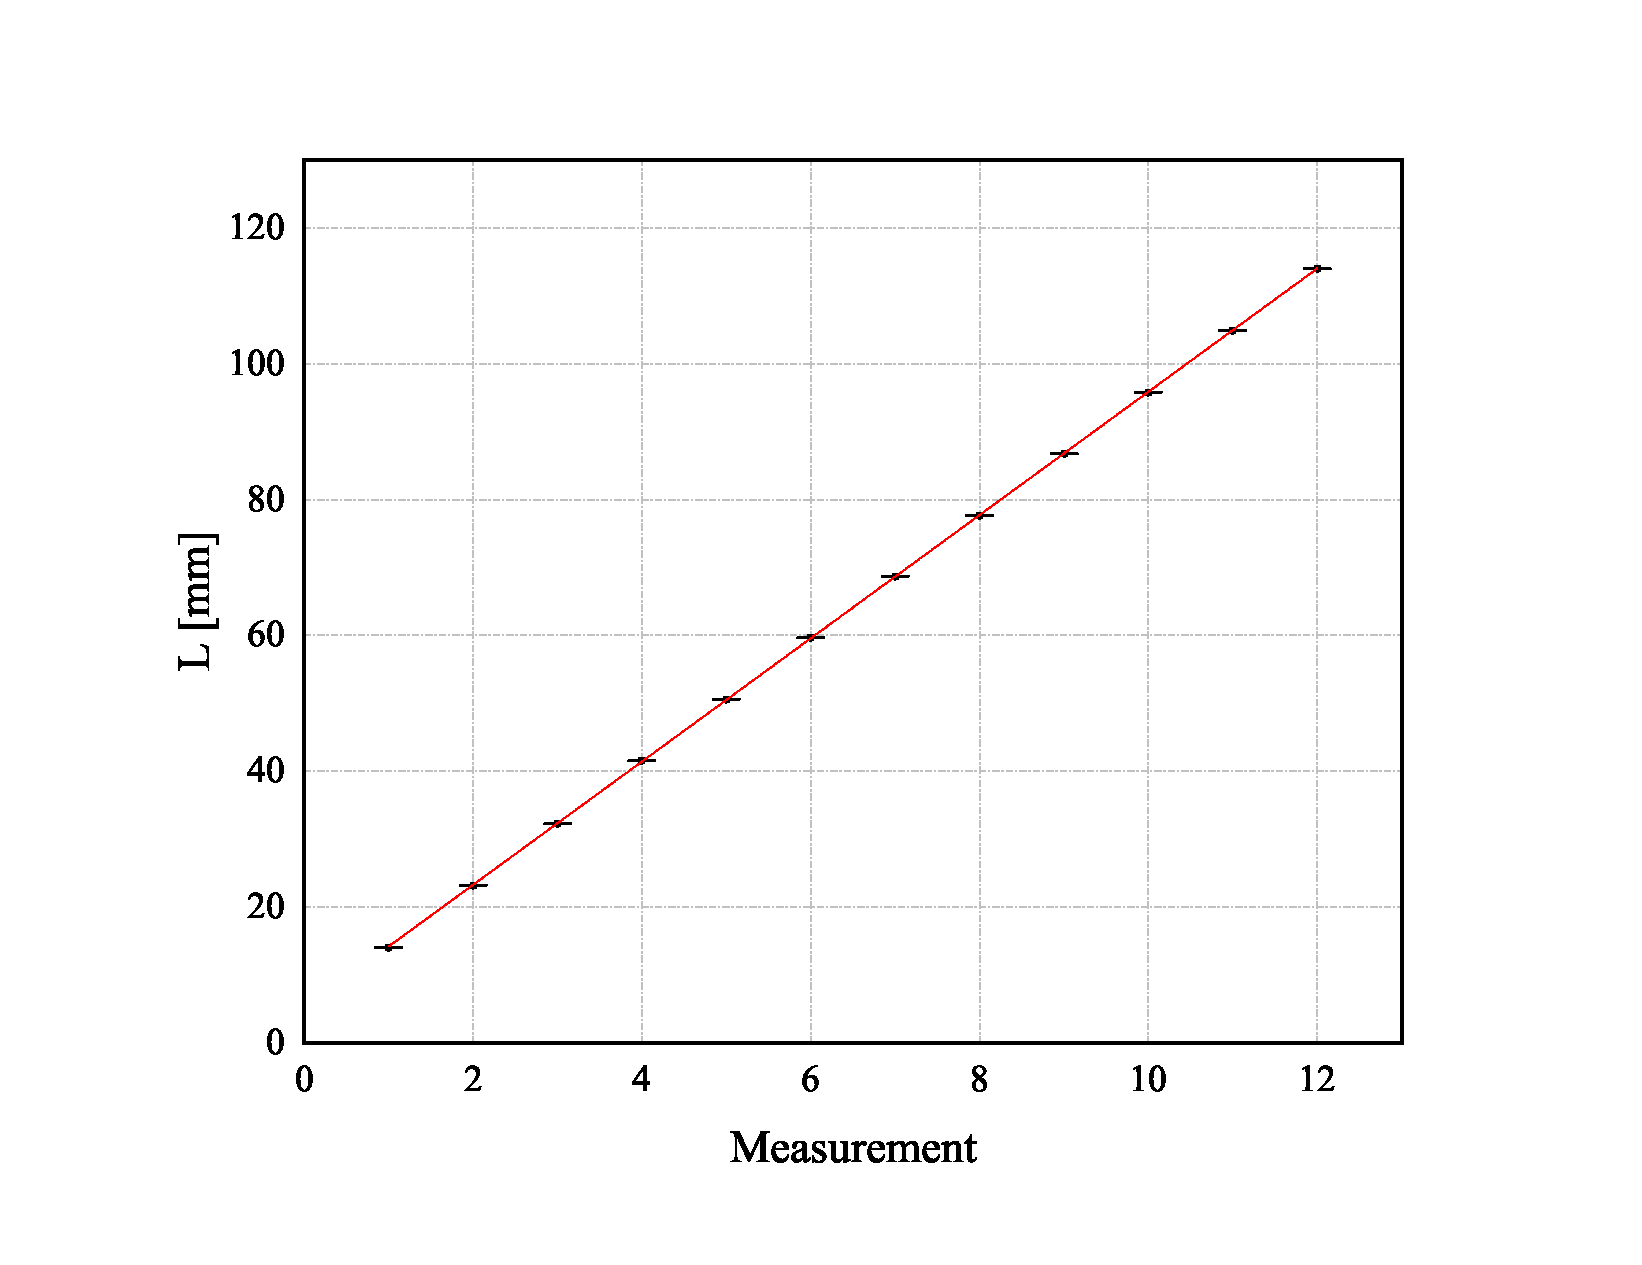
\includegraphics[width=0.8\linewidth]{3.eps}
		\caption{Measurement data with error bars and a linear fit to the data for the relation between the distance and the measurement. The value of $R^2$ for the obtained fit is 0.99999.}
		\label{fig:3}
	\end{figure}
	\subsection{Measurements of the speed of sound by time- difference method (liquid)}
	The distances between $S_1$ and $S_2$ $L_i$ and corresponding time period $t_i$ were measured in the procedure described in section 3.3 and the linear fit can be derived from Table 3.
	\begin{tabular}{|c|c|c|}
		\hline
		Measurement&$t_i$ [$\mu$s]$\pm$0.02[$\mu$s]&$L_i$[mm]$\pm$0.001[mm]\\
		\hline
		1&74.0&100.000\\
		\hline
		2&79.6&110.000\\
		\hline
		3&86.8&120.000\\
		\hline
		4&93.6&130.000\\
		\hline
		5&100.4&140.000\\
		\hline
		6&106.8&150.000\\
		\hline
		7&113.6&160.000\\
		\hline
		8&120.4&170.000\\
		\hline
		9&127.2&180.000\\
		\hline
		10&134.0&190.000\\
		\hline
		11&140.0&200.000\\
		\hline
		12&147.0&210.000\\
		\hline
	\end{tabular}
	\begin{center}
		Table 2. Data table for the phase comparison method.
	\end{center}
	By Equation 2, the value of the distance $L$ is linear to the time span $t$, which is presented in Figure 4. Having determined a proper statistical test that indicates linear relation, we fit a straight line $L=\alpha t+\beta$ to the data. By linear fitting, the slope $\alpha=1.496\ \rm{mm/\mu s}$ and the intercept $\beta=-9.957$ mm with standard errors $u_\alpha=0.006\ \rm{mm/\mu s}$ mm and $u_\beta=0.644$ mm and $R^2$=0.99985. The fitting procedure are performed using Origin.
	Using the value of the slope from the linear relation Equation 3, the speed of sound $v$ can be found as
	\begin{equation}
	v=\alpha=1496\pm6\ \rm{m/s}
	\end{equation}
	with the relative uncertainty 0.40\%.
	\begin{figure}[H]
		\centering
		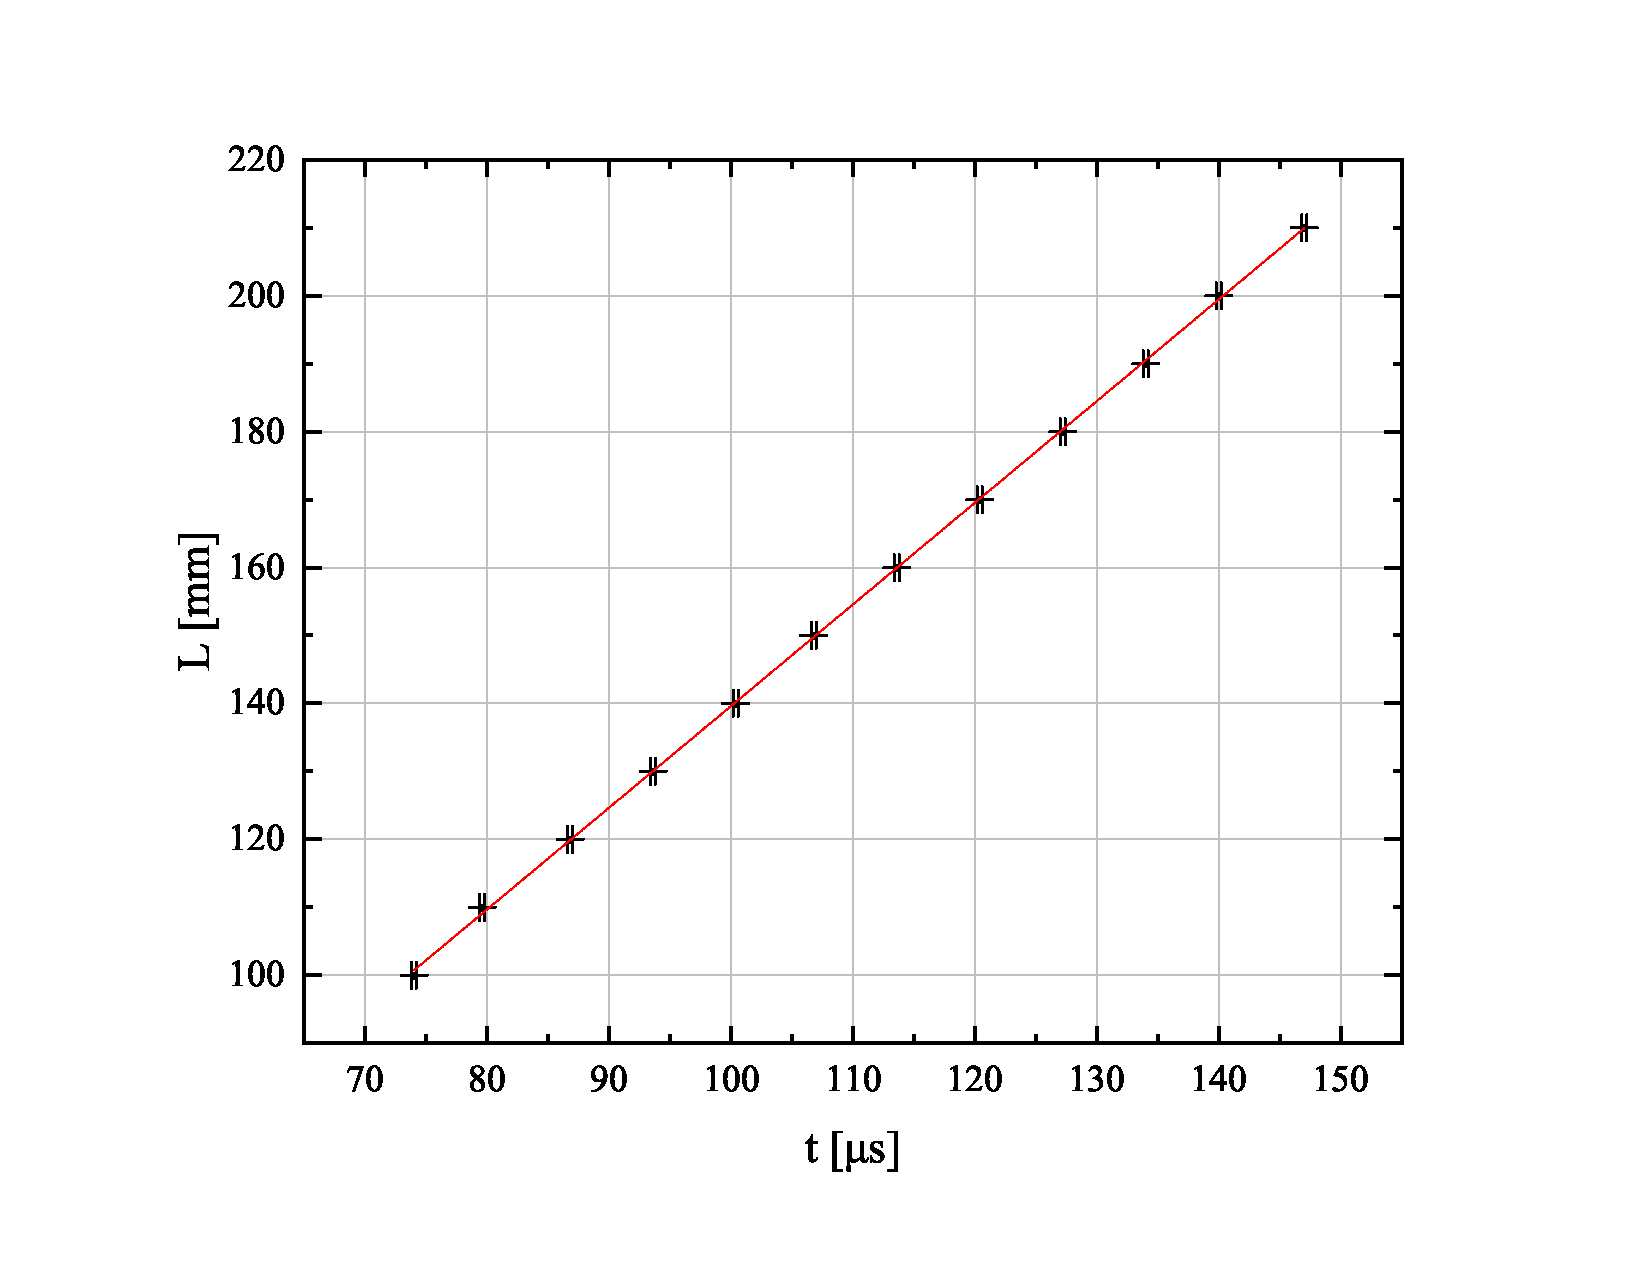
\includegraphics[width=0.8\linewidth]{4.eps}
		\caption{Measurement data with error bars and a linear fit to the data for the relation between the distance and the time period. The value of $R^2$ for the obtained fit is 0.99985.}
		\label{fig:4}
	\end{figure}
	\section{Conclusions and discussion}
	In this experiment, the sound of speed is measured by three methods, having $L$ vs. $n$, $L$ vs. $n$, and $L$ vs. $t$ lines respectively. The former two methods are used to measure the sound of speed in air while the last one method is used to measure the sound of speed in water. Comparing the results of the former two methods,
	\begin{equation*}
	v=351.043\pm0.693\ \rm{m/s} \qquad \rm{and} \qquad 349.195\pm0.270\ \rm{m/s,}
	\end{equation*}
	respectively, with the later method yielding smaller uncertainty. Compared with the speed of sound $v_1=343.21\ \rm{m/s}$ at $20^\circ {\rm C}$ and $v_2=346.13\ \rm{m/s}$ at $25^\circ {\rm C}$, both values are slightly higher than is expected quoted for “Speed of sound.” \textit{Wikipedia}. Wikimedia Foundation, 5 June. 2019. Web. 23 June. 2019.
	
	Reviewing the trend of the speed of sound as temperature, we find that it generally increases as temperature increases in air so that a range is formed while the measured data does not fall in the range. The source of inaccuracy of both methods is that the determining point on the oscilloscope is sensitive to the interference of the noises and infinitesimal change of the distance between $S_1$ and $S_2$.
	
	The precision of the measurements can be further determined by the returning motion of $S_2$ during any part of the experiment that will cause the backslash error. When turning the rotary knob on the micrometer caliper, the graph is not stable and it is impossible to know the maximum value before it is missed a little so that neither a backslash nor a lower value than the maximum value behind is avoidable. Besides, the middle line on the major scale of the caliper is not marked straightly so that the reading may not be accurate.
	
	Compared with the former two methods, the last method is quite direct but actually introduces higher error since the precision of the time is $0.2\ \mu\rm{s}$, which is much higher than that of the distance $L$, as the electronic sensor is endowed with time measurement error. Comparing the experimental result $v_1$ to the referred result $v_2$ quoted for "Speed of Sound in Water at Temperatures between 32–212 oF (0–100 oC) — imperial and SI units". \textit{The Engineering Toolbox}.,
	\begin{equation*}
	v_1=1496\pm6\ \rm{m/s} \qquad \rm{and} \qquad v_2=1481\ \rm{m/s}
	\end{equation*}
	which is also a slightly higher, indicating the reason for the inaccuracy discussed above.
	\newpage
	\renewcommand\thesection{\Alph{section}}
	\setcounter{section}{0}
	\section{Measurement uncertainty analysis}
	\subsection{Uncertainty of distance measurements}
	Since the measurements of the distance between $S_1$ and $S_2$ are single measurements and the type-B uncertainty is 0.001 mm, the uncertainty of distance measurements is
	\begin{equation*}
	u_L=1\times 10^{-6}\ \rm{m}
	\end{equation*}
	\subsection{Uncertainty of time measurements}
	Since the measurements of the time when signals are trasmitted from $S_1$ to $S_2$ are single measurements and the type-B uncertainty is 0.2 $\mu$s, the uncertainty of distance measurements is
	\begin{equation*}
	u_t=2\times 10^{-7}\ \rm{s}
	\end{equation*}
	\subsection{Uncertainty of wavelength measurements}
	By the resonance method, according to Equation 1 and Equation 3, we have know
	\begin{equation*}
	v=\dfrac{2Lf}{n}
	\end{equation*}
	the uncertainty $u_v$ can be found by applying the uncertainty propagation formula
	\begin{equation*}
	u_v=\sqrt{\dfrac{\partial v}{\partial L}^2 u_L^2+\dfrac{\partial v}{\partial f}^2 u_f^2+\dfrac{\partial v}{\partial n}^2 u_n^2}
	\end{equation*}
	Since $u_f=u_n=0$ and the average measurement
	\begin{equation*}
	\bar{n}=\dfrac{\sum_{i=1}^{12}i}{12}=6.5
	\end{equation*}
	we have
	\begin{equation*}
	u_v=\dfrac{\partial v}{\partial L} u_L=\dfrac{2f}{\bar{n}} u_L=0.107 \rm{m/s}
	\end{equation*}
	
	Hence, the value of the speed of sound in air is
	\begin{equation*}
	v=351.043\pm0.107\ \rm{m/s}
	\end{equation*}
	with the relative uncertainty 0.03%.
	
	Similarly, by the phase difference method, we have
	\begin{equation*}
	v=\dfrac{Lf}{\bar{n}}
	\end{equation*}
	Then,
	\begin{equation*}
	u_v=\dfrac{\partial v}{\partial L} u_L=\dfrac{f}{\bar{n}} u_L=0.041 \rm{m/s}
	\end{equation*}
	
	Hence, the value of the speed of sound in air is
	\begin{equation*}
	v=349.195\pm0.041\ \rm{m/s}
	\end{equation*}
	with the relative uncertainty 0.01%.
	\subsection{Uncertainty of the speed of sound found from the slope of the $L$ vs. $t$ line}
	The uncertainty of the speed of sound found from the slope of the $L$ vs. $t$ line can be estimated by the uncertainty of the slope $\alpha$ calculated when fitting $u_\alpha=0.006 \rm{m/s}$. Then, the speed of sound is directly equal to the slope $\alpha$.
	\begin{equation*}
	u_v=u_\alpha=0.006\ \rm{mm/\mu s}=6\ \rm{m/s}
	\end{equation*}
	
	Hence, the value of the speed of sound that is found rom the slope of the fitting line is equal to
	\begin{equation*}
	v=1496\pm6\ \rm{m/s}
	\end{equation*}
	with the relative uncertainty 0.40%.
	\section{Data Sheet}
	\begin{figure}[H]
		\centering
		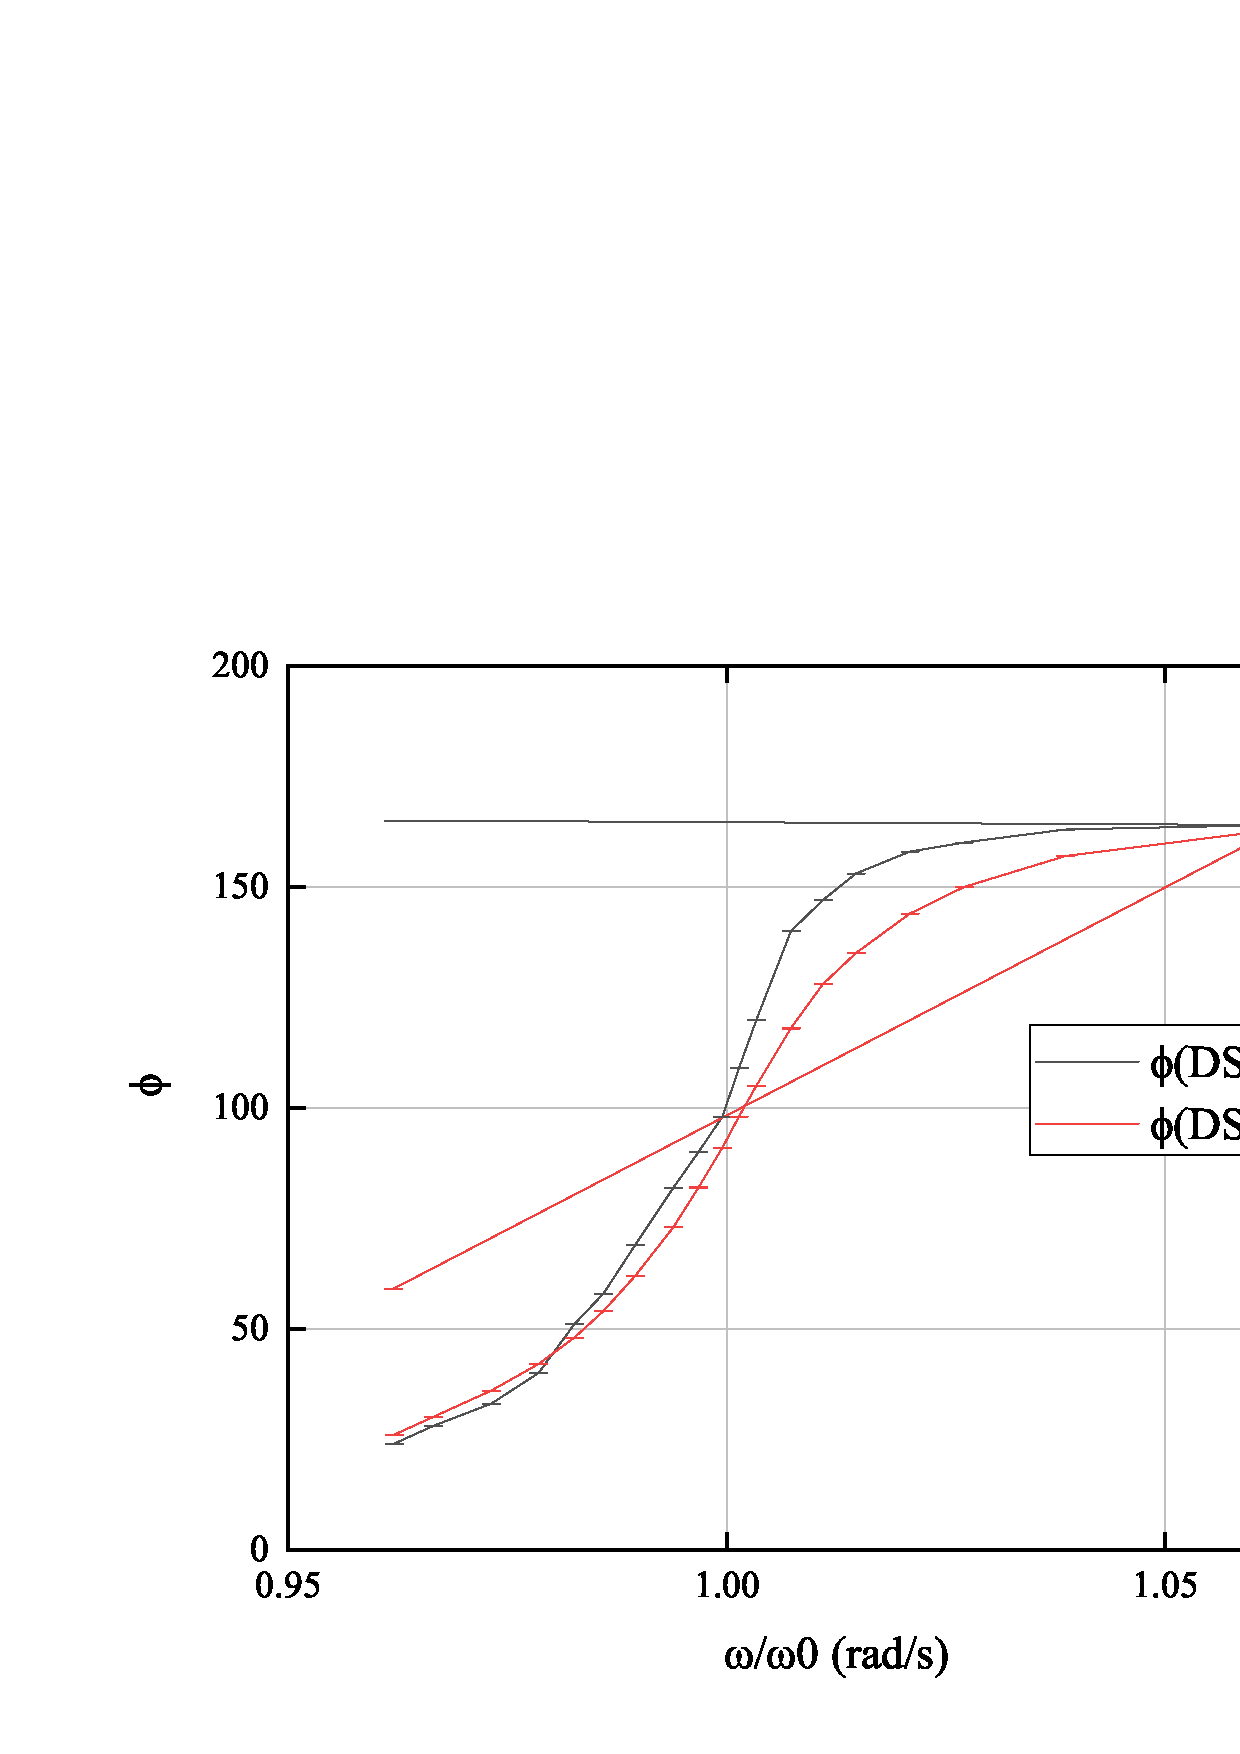
\includegraphics[width=1\linewidth]{5.jpg}
	\end{figure}
	\begin{figure}[H]
		\centering
		\includegraphics[width=1\linewidth]{6.jpg}
	\end{figure}
\end{document}